\everymath{\displaystyle}
\documentclass{beamer}
% \documentclass[handout]{beamer}

%\usepackage[pdftex]{color,graphicx}
\usepackage{amsmath,amssymb,amsfonts}

\mode<presentation>
{
  % \usetheme{Darmstadt}
  % \usetheme[hideothersubsections]{Hannover}
  % \usetheme[hideothersubsections]{Goettingen}
  \usetheme[hideothersubsections, right]{Berkeley}

  \usecolortheme{seahorse}
  % \usecolortheme{dolphin}
  \usecolortheme{rose}
  % \usecolortheme{orchid}

  \useinnertheme[shadow]{rounded}

  \setbeamercovered{transparent}
  % or whatever (possibly just delete it)
}

\mode<handout>{
  \setbeamercolor{background canvas}{bg=black!5}
  \usepackage{pgfpages}
  \pgfpagesuselayout{4 on 1}[a4paper,border shrink=5mm, landscape]
}

\usepackage[brazilian]{babel}
% or whatever

% \usepackage[latin1]{inputenc}
\usepackage[utf8]{inputenc}
% or whatever

\usepackage{times}
%\usepackage[T1]{fontenc}
% Or whatever. Note that the encoding and the font should match. If T1
% does not look nice, try deleting the line with the fontenc.


\title[Revisão 1] % (optional, use only with long paper titles)
{Revisão (parte 1)}

\subtitle
{Probabilidade e Estatística} % (optional)

\author%[] % (optional, use only with lots of authors)
{Felipe Figueiredo}% \and S.~Another\inst{2}}
% - Use the \inst{?} command only if the authors have different
%   affiliation.

\institute[UNIAN] % (optional, but mostly needed)
{UNIAN - Centro Universitário Anhanguera de Niterói
}
  % \inst{1}%
  % Department of Computer Science\\
  % University of Somewhere
  % \and
  % \inst{2}%
  % Department of Theoretical Philosophy\\
  % University of Elsewhere}
% - Use the \inst command only if there are several affiliations.
% - Keep it simple, no one is interested in your street address.

\date%[] % (optional)
{}

% \subject{Talks}
% This is only inserted into the PDF information catalog. Can be left
% out. 



% If you have a file called "university-logo-filename.xxx", where xxx
% is a graphic format that can be processed by latex or pdflatex,
% resp., then you can add a logo as follows:

\pgfdeclareimage[height=1.6cm]{university-logo}{../logo}
\logo{\pgfuseimage{university-logo}}



% Delete this, if you do not want the table of contents to pop up at
% the beginning of each subsection:
\AtBeginSubsection[]
%\AtBeginSection[]
{
  \begin{frame}<beamer>{Sumário}
    \tableofcontents[currentsection,currentsubsection]
  \end{frame}
}


% If you wish to uncover everything in a step-wise fashion, uncomment
% the following command: 

\beamerdefaultoverlayspecification{<+->}


\begin{document}

\begin{frame}
  \titlepage
\end{frame}

% \begin{frame}{Sumário}
%   \tableofcontents
%   % You might wish to add the option [pausesections]
% \end{frame}


%% Template
% \section{}

% \subsection{}

% \begin{frame}{}
%   \begin{itemize}
%   \item 
%   \end{itemize}
% \end{frame}

% \begin{frame}
%   \begin{columns}
%     \begin{column}{5cm}
%     \end{column}
%     \begin{column}{5cm}
%     \end{column}
%   \end{columns}
% \end{frame}

% \begin{frame}{}
%   \includegraphics[height=0.4\textheight]{file1}
%   \includegraphics[height=0.4\textheight]{file2}
%   \includegraphics[height=0.4\textheight]{file3}
%   \begin{figure}
%     \caption{}
%   \end{figure}
% \end{frame}

% \begin{frame}{}
%   \begin{definition}
%   \end{definition}
%   \begin{example}
%   \end{example}
%   \begin{block}{Exercício}
%   \end{block}
% \end{frame}


\begin{frame}{Matéria 1 de jornal}
Considere a seguinte matéria recente de jornal:

\bigskip
\bigskip
\bigskip
\centering 
\includegraphics[width=.9\textwidth]{Revisao1/manchete}

\vfill
Fonte: Folha de São Paulo, 19/03/2016
\end{frame}

\begin{frame}{Início}
  \centering 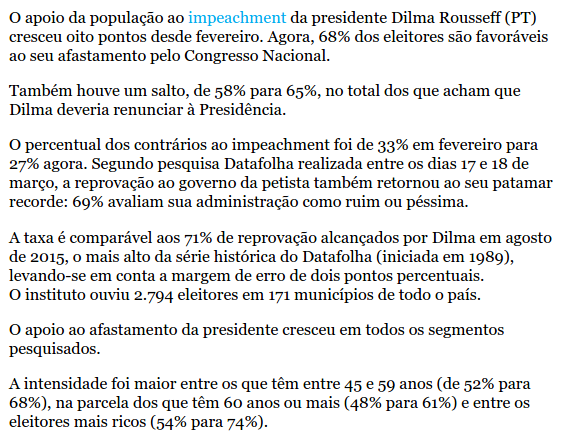
\includegraphics[height=.9\textheight]{Revisao1/texto}
\end{frame}

\begin{frame}{Trecho}
  \begin{quote}
    O apoio da população ao impeachment da presidente Dilma Rousseff
    (PT) cresceu oito pontos desde fevereiro. Agora, 68\% dos
    eleitores são favoráveis ao seu afastamento pelo Congresso
    Nacional [\ldots]. O instituto [Datafolha] ouviu 2.794 eleitores em 171
    municípios de todo o país.
  \end{quote}
  \begin{block}{Perguntas}
    \begin{itemize}
    \item Este estudo foi feito com uma população, ou com uma amostra?
    \item As porcentagens acima são parâmetros ou estatísticas?
    \item Qual é a população deste estudo?
    \end{itemize}
  \end{block}
\end{frame}

\begin{frame}{Matéria 2 de jornal}
Considere a seguinte matéria recente de jornal:

\bigskip
\bigskip
\bigskip
\centering 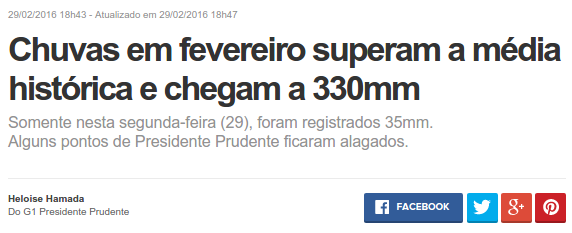
\includegraphics[width=.9\textwidth]{Revisao1/manchete2}

\vfill
Fonte: G1 Presidente Prudente, 29/02/2016
\end{frame}

\begin{frame}{Início}
  \centering 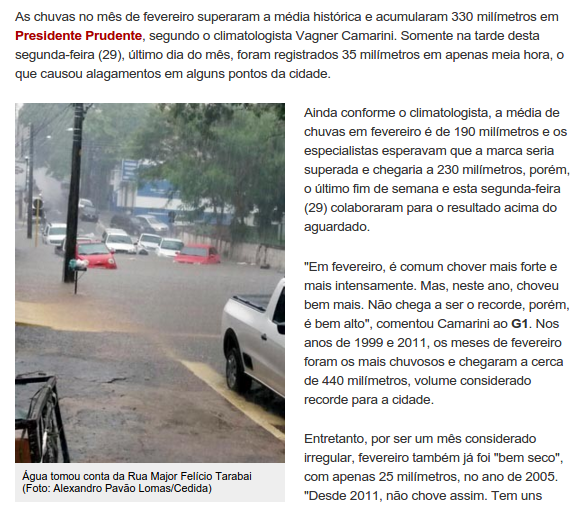
\includegraphics[height=.9\textheight]{Revisao1/texto2}
\end{frame}

\begin{frame}{Trecho}
  \begin{quote}
    As chuvas no mês de fevereiro superaram a média histórica e
    acumularam 330 milímetros em Presidente Prudente, segundo o
    climatologista Vagner Camarini. [\ldots] a média de chuvas em
    fevereiro é de 190 [mm] e os especialistas esperavam que a
    marca seria superada e chegaria a 230 [mm] [\ldots]
  \end{quote}
  \begin{block}{Perguntas}
    \begin{itemize}
    \item O resultado apresentado é um parâmetro ou estatística?
    \item Qual é a população deste estudo?
    \item Além da média, que outra medida sumária seria necessária
      para uma descrição completa dos dados?
    \end{itemize}
  \end{block}
\end{frame}

\begin{frame}{Reprodução dos dados}
  \centering 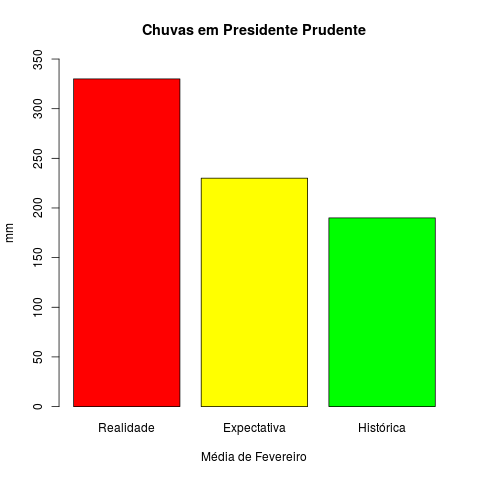
\includegraphics[height=.85\textheight]{Revisao1/materia2}

Houve um aumento de chuva neste fevereiro?
\end{frame}

\end{document}
